\documentclass[12pt, twoside]{article}
\usepackage[letterpaper, margin=1in, head=30pt, headsep=0.1in]{geometry}
\usepackage[english]{babel}
\usepackage[utf8]{inputenc}
\usepackage{amsmath}
\usepackage{amsfonts}
\usepackage{amssymb}
\usepackage{tikz}
%\usetikzlibrary{quotes, angles}

\usepackage{graphicx}
\usepackage{enumitem}
\usepackage{multicol}

\newif\ifmeta
\metatrue %print standards and topics tags

\title{Regents Geometry}
\author{Chris Huson}
\date{October 2021}

\usepackage{fancyhdr}
\pagestyle{fancy}
\fancyhf{}
\renewcommand{\headrulewidth}{0pt} % disable the underline of the header
\raggedbottom


\fancyhead[LE]{\thepage}
\fancyhead[RO]{\thepage \\ Name: \hspace{4cm} \,\\}
\fancyhead[LO]{BECA / Dr. Huson / Geometry 04 Analytic Geometry}

\begin{document}

\subsubsection*{4.3 Partitioning a line segment}
The distance formula: $\displaystyle d=\sqrt{(x_2-x_1)^2+(y_2-y_1)^2}$
\begin{enumerate}
\item Do Now: Dr. Huson's commute is from 80th Street to 164th Street. 
\begin{enumerate}
  \item On what block is he half way? Mark it and label it with the street number.
  \item On the way to work, mark and label the block when he is three-quarters of the way to BECA.
\end{enumerate}
  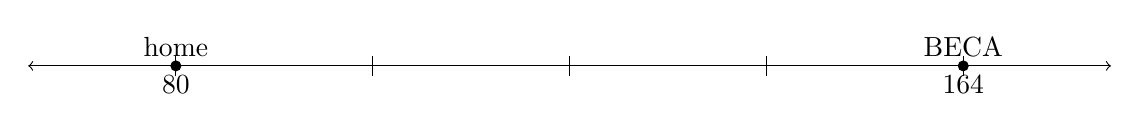
\begin{tikzpicture}[scale=1.25]
    \draw [<->] (-4.5,0)--(6.5,0);
    \foreach \x in {-3,-1,...,5} %2 leading for diff!=1
      \draw[shift={(\x,0)},color=black] (0pt,-3pt) -- (0pt,3pt);% node[below=5pt]  {$\x$};
      \draw [fill] (-3,0) circle [radius=0.05] node[above] {home};
      \draw [fill] (5,0) circle [radius=0.05] node[above] {BECA};
      \node at (-3,0) [below]{80};
      \node at (5,0) [below]{164};
  \end{tikzpicture}
  \vspace{5cm}

  \item On the graph, draw polygon ABCDEF with vertices A(1, 1), B(1, 4), C(3, 4), D(3, 7), E(8, 7), and F(8, 1). Find the perimeter and the area of the polygon.
  \begin{flushleft}
    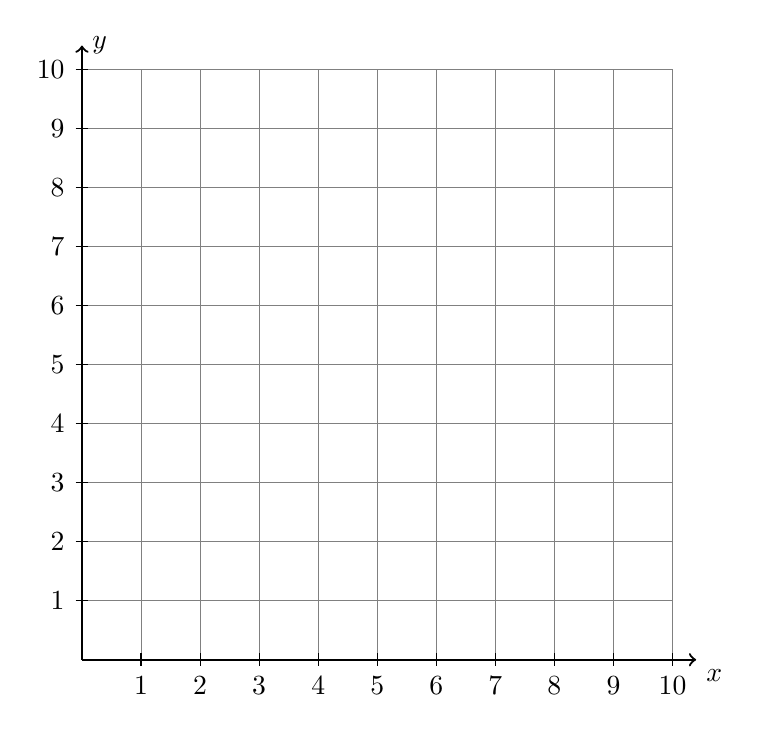
\begin{tikzpicture}[scale=.75]
      \draw [help lines] (0,0) grid (10,10);
      \draw [thick, ->] (0,0) -- (10.4,0) node [below right] {$x$};
      \draw [thick, ->] (0,0)--(0,10.4) node [right] {$y$};
      \foreach \x in {1,...,10}
      \draw[shift={(\x,0)}] (0pt,-3pt)--(0pt,3pt) node[below=5pt] {$\x$};
      \foreach \y in {1,...,10}
      \draw[shift={(0,\y)}] (-3pt,0pt)--(3pt,0pt) node[left=5pt] {$\y$};
    \end{tikzpicture}
    \end{flushleft}
  \vspace{2cm}

\newpage
\item In the diagram below, $\overline{AB}$ has endpoints with coordinates $A(-3,4)$ and $B(5, -2)$.
\begin{enumerate}
  \item Find the coordinates of the midpoint $M$ of $\overline{AB}$. Mark and label it on the graph.
  \item Find the length $AB$
\end{enumerate}

  \begin{flushright} %4 quadrant regents grid
    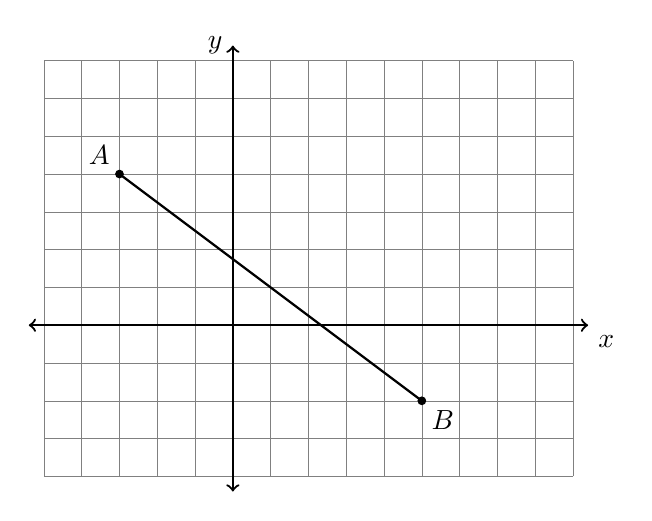
\begin{tikzpicture}[scale=.48]
      \draw [help lines] (-5,-4) grid (9,7);
      \draw [thick, <->] (-5.4,0) -- (9.4,0) node [below right] {$x$};
      \draw [thick, <->] (0,-4.4)--(0,7.4) node [left] {$y$};
      \draw [thick] (-3,4)--(5, -2);
      \draw [fill] (-3,4) circle [radius=0.1] node[above left] {$A$};
      \draw [fill] (5, -2) circle [radius=0.1] node[below right] {$B$};
    \end{tikzpicture}
  \end{flushright}

\item Find each pair of numbers with the given sum.
\begin{enumerate}
  \item Example: Two numbers with a ratio of $3:1$ that sum to 20 are $15:5$.
  \item $2:1$, sum 9 \vspace{1cm}
  \item $1:1$, sum 100 \vspace{1cm}
  \item $2:3$, sum 20 \vspace{1cm}
\end{enumerate}

\item Divide (partition) $\overline{AB}$, $A=-3$ and $B=6$, into three equal parts. Mark and label the dividing points $P$ and $Q$. \\
  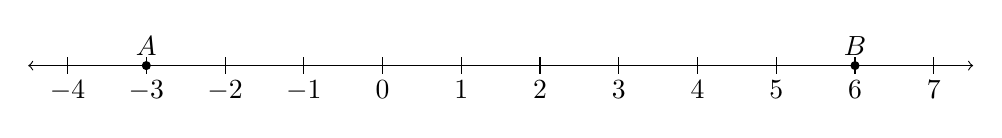
\begin{tikzpicture}
    \draw [<->] (-4.5,0)--(7.5,0);
    \foreach \x in {-4,...,7} %2 leading for diff!=1
      \draw[shift={(\x,0)},color=black] (0pt,-3pt) -- (0pt,3pt) node[below=5pt]  {$\x$};
      \draw [fill] (-3,0) circle [radius=0.05] node[above] {$A$};
      \draw [fill] (6,0) circle [radius=0.05] node[above] {$B$};
  \end{tikzpicture}
  \vspace{0.5cm}

  \item Partition $\overline{MN}$, $M=-3$ and $N=5$, in the ratio $3:1$ with point $P$. \\
  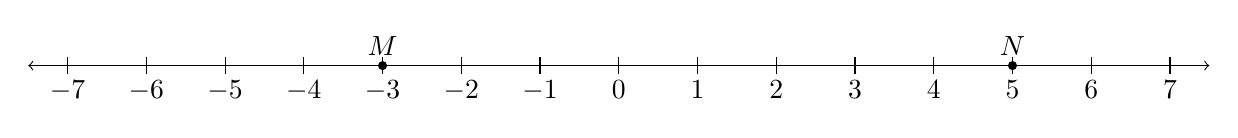
\begin{tikzpicture}
    \draw [<->] (-7.5,0)--(7.5,0);
    \foreach \x in {-7,...,7} %2 leading for diff!=1
      \draw[shift={(\x,0)},color=black] (0pt,-3pt) -- (0pt,3pt) node[below=5pt]  {$\x$};
      \draw [fill] (-3,0) circle [radius=0.05] node[above] {$M$};
      \draw [fill] (5,0) circle [radius=0.05] node[above] {$N$};
  \end{tikzpicture}

\end{enumerate}
\end{document}
